\section{Einführung}
Der Autor arbeitet als GIS-Spezialist bei der swisstopo\footnote{\href{https://www.swisstopo.ch}{www.swisstopo.ch}}, dem Bundesamt für Landestopografie, in Wabern.\\ Unter anderem macht die swisstopo Karten. Das Team des Autoren macht Internetkarten. Lieber Leser\footnote{Im vorliegenden Dokument wurde primär eine geschlechterneutrale Formulierungen angewandt. Wo es sich nicht vermeiden liess, wurde durchwegs der männliche Singular (Leser, Benutzer) als Ansprache verwendet. Diese Ansprache bezieht sich auf beide Geschlechter sowie gegebenenfalls mehrere Personen. Sie dient lediglich der leichteren Lesbarkeit der Semesterarbeit.}, falls dir \href{https://map.geo.admin.ch}{map.geo.admin.ch} noch kein Begriff sein sollte, kann wärmstens empfohlen werden, darin zu schmökern. Die Internetkarte erfreut sich relativ grosser Beliebtheit und beinhaltet ca. 800 Themen wie Wanderwege, Solarkataster und Luftfahrthindernisse. Die Karte und die dazugehörenden Web Services sind gratis - ein Service Public der Schweizerischen Bundesverwaltung.

\begin{figure}[H]
	\centering
	\href{https://s.geo.admin.ch/8a82499889}{
	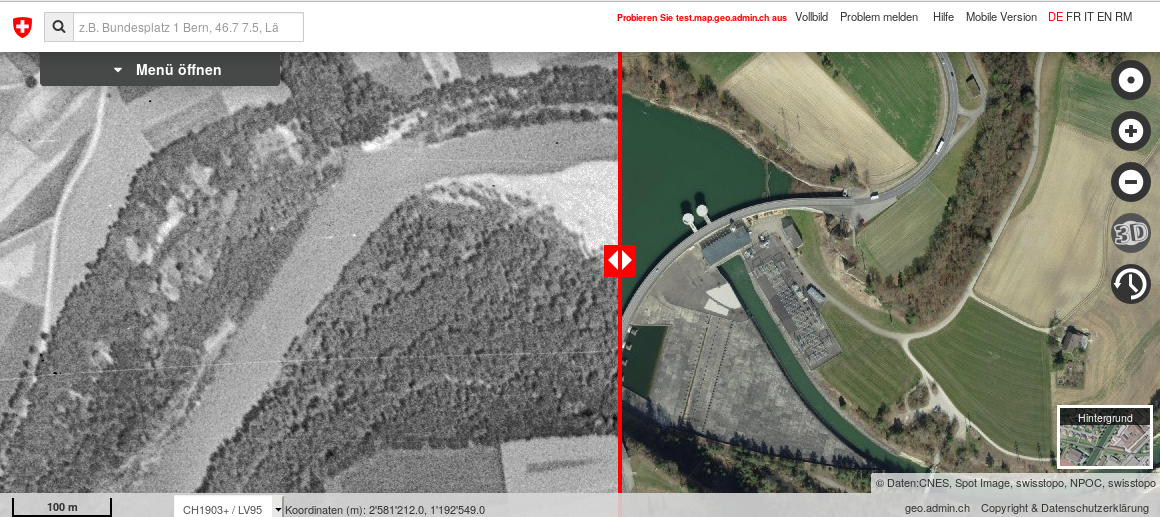
\includegraphics[width=.80\textwidth]{hist_map_geo_admin}}
	\caption{Internetkarte des Bundes \emph{\href{https://s.geo.admin.ch/8a82499889}{map.geo.admin.ch}}. Hier ein Ausschnitt der Saane bei Kleinbösingen, das Luftaufnahmen von 1946 mit heute vergleicht.}
	\label{fig:map.geo.admin.ch}
\end{figure}


\subsection{GIS - Geografische Informationssysteme}
Wie erwähnt, arbeitet der Autor als \emph{GIS-Spezialist}. Wobei ihm der Titel \emph{Geoinformatiker} besser gefällt: weil dieser Titel die Begriffe \emph{Geografie} und \emph{Informatik} vereint. \emph{Geografie} kommt aus dem Griechischen und bedeutet Erdbeschreibung \autocite[14]{Schertenleib2004}. \emph{Informatik} ist die Wissenschaft von der systematischen Darstellung, Speicherung, Verarbeitung und Übertragung von Informationen \cite{Informatik2010}.

GIS ist ein Akronym für Geografische Informationssysteme. Es bedeutet im engsten Sinn eine Ansammlung von Computerprogrammen, die zur Bearbeitung von Karten und Geodaten verwendet werden. Geodaten sind nichts weiter als Daten mit einem räumlichen Bezug\footnote{Mit Koordinaten (Nord/Ost, x/y).}. In einem weiteren Sinn deckt der Begriff GIS ein ganzes Fachgebiet ab, das sich mit Karten und Geodaten auskennt. Es ist also nicht nur ein Werkzeug, sondern ein Fachgebiet, das Kenntnisse über Datensammlung, Speicherung, Analyse und Darstellung innerhalb von vielen verschiedenen Themen mit einem räumlichen Bezug abdeckt. Typische Geodaten sind digitale Karten, Inventare und Register von Parzellen, Umweltfaktoren, Grenzen, Entwicklung, Planung etc., die einen räumlichen Bezug haben und dadurch in einem geografischen Zusammenhang analysiert und dargestellt werden können \autocite[15]{Balstroem}.

Es ist zwar weit von der klassischen Geografie zu Zeiten Alexanders von Humbold\footnote{Ein Forschungsreisender des 19 Jh. mit einem weit über Europa hinausreichenden Wirkungsfeld. Mehrjährige Forschungsreisen führten ihn nach Lateinamerika, USA und nach Zentralasien \cite{Kehlmann2005}.} entfernt, aber es liegt auf der Hand, dass auch die Geografie Cloud Computing nutzt.